%%%%%%%%%%%%%%%%%%%%%%%%%%%%%%%%%%%%%%%%%%%%%%%%%
%%%%%%%%%%%%%%%%%%%%%%%%%%%%%%%%%%%%%%%%%%%%%%%%%

1\chapter{Experimental Setup}
\label{chap:third}

%%%%%%%%%%%%%%%%%%%%%%%%%%%%%%%%%%%%%%%%%%%%%%%%%
%%%%%%%%%%%%%%%%%%%%%%%%%%%%%%%%%%%%%%%%%%%%%%%%%

This chapter describes the experimental setup for the simulations that were performed, for the purpose of this study. Section~\ref{chap:robots} describes the robots used in the study, and the simulation environment is described in Section~\ref{simulator}. The environments used in the experiment are discussed in Section~\ref{experimentenvironments}, while Section~\ref{parameters} defines the parameters for the robot swarm. Section~\ref{thri:third:performancemeasures} defines the performance measures used to evaluate the results of the experiments. The chapter is summarized in Section~\ref{third:summary}.

%%%%%%%%%%%%%%%%%%%%%%%%%%%%%%%%%%%%%%%%%%%%%%%%%
%%%%%%%%%%%%%%%%%%%%%%%%%%%%%%%%%%%%%%%%%%%%%%%%%

\section{Robots}
\label{chap:robots}

Foraging robots occur in all shapes, sizes and capabilities. Some robots have powerful GPS capabilities and advanced long distance sensors, while others are much simpler. This chapter defines the capabilities of the simulated robots to be used in this study. The robots are described in Section~\ref{robotdescription}, while Section~\ref{navigationandobstacleavoidance} outlines the navigational capabilities of the robots. Section~\ref{simulator} discusses the simulator used.

\subsection{Robot Description}
\label{robotdescription}

The artificial robots modelled in this study are based on e-puck robots \cite{mondada2009puck}, adapted with grippers. A robot is equipped with a 360 degree camera to identify objects around the robot, as well as eight local distance sensors spaced equally around the circular perimeter of the robot. Both camera and distance sensors have a depth of view of five times the robot's size. Robots use local communication which can occur in a radius of five times the robot's size. On real robots, the local communication could occur via use of light signals or ZigBee communications. The sensor and communication range is sufficiently localized with respect to the size of the environment. A robot can forage a single item at a time. The robots do not have a global positioning system (GPS) capability to locate items to position themselves in the environment. A robot cannot see an item hidden by another item. As a result, robots have to explore the environment to find the prioritized items.

\subsection{Navigation and Obstacle Avoidance}
\label{navigationandobstacleavoidance}

The environments used in the simulation have a variety of complexities: Some environments are very sparse, while others have large zones of items that must be navigated around. Due to the environmental complexity, an advanced navigation and obstacle avoidance technique is required. 

The robots in the experiments, in this thesis, use a navigation and obstacle avoidance technique inspired by an approach developed for communication congestion avoidance in wireless sensor networks \cite{antoniou2012congestion}. Antoniou et al. use inspiration from the flocking behaviour of birds, in order to efficiently route messages around communication congestion in wireless sensor networks. In flocking behaviour of birds, birds are attracted by a global magnetic attractor to the birds final destination, while a local attractor pulls flocking birds away from areas of congestion. In the congestion avoidance algorithm, the final destination of the message being sent on the wireless sensor network is the global attractor while a local attractor pulls the message around congested areas.

The described congestion avoidance technique has been adapted to form a simple but effective navigation and obstacle avoidance technique. Robots are pulled to a global attractor which is the intended destination, while a local attractor directs robots away from local obstacles while maintaining a course to the destination.

Figure \ref{fig:obstacleavoidance} illustrates the navigation and obstacle avoidance method used by the robots. The navigation and obstacle avoidance algorithm achieves the effect of the global attractor by setting the robots field of view towards the direction to the desired destination. The destination is determined by a homing beacon or by the robot's path integration vector. The direction at the centre of the field of view is the direction to the destination. 

The effect of the local attractor is modelled by  evaluating each direction in the field of view, to select the most desirable direction. Desirability, $d$, of a direction, $i$, is a metric quantifying the how well a direction achieves a balance between clarity of the path and directness of the direction to the destination. The clarity, $\kappa_i$, in a direction $i$, is a normalized reading from the proximity sensor or camera such that $\kappa_i\in[0,1]$. Clarity indicates the distance of next nearest obstacle. If no obstacles exist in the depth of view $v$, then  $\kappa_i=0$ and if there exists an obstacle immediately next to the robot, then $\kappa_i=0=1$. The directness of a direction $i$, $\iota_i\in[0,1]$ is calculated as the angular deviation from the direction of the destination, where $\iota_i=0$ occurs when the direction $i$ is the same as direction to the destination, $dir$, and a $\iota_i=1$ occurs when the direction is at the edge of the field of view, $f$. Desirability $d_i$ of direction $i$ is defined mathematically in Equation \ref{eq:1}.

\begin{equation}
	d_i= \lambda \kappa_i + (1 - \lambda)\iota_i \\
	\label{eq:1}
\end{equation} where $\lambda$ determines whether clarity, $c_i$ or directness, $\iota_i$ of direction $i$, has more effect on desirability. The described navigation and obstacle avoidance technique is used with all algorithms in the experiment and for algorithms $\lambda$ is set to 0.5.

\begin{figure}
	\centering
	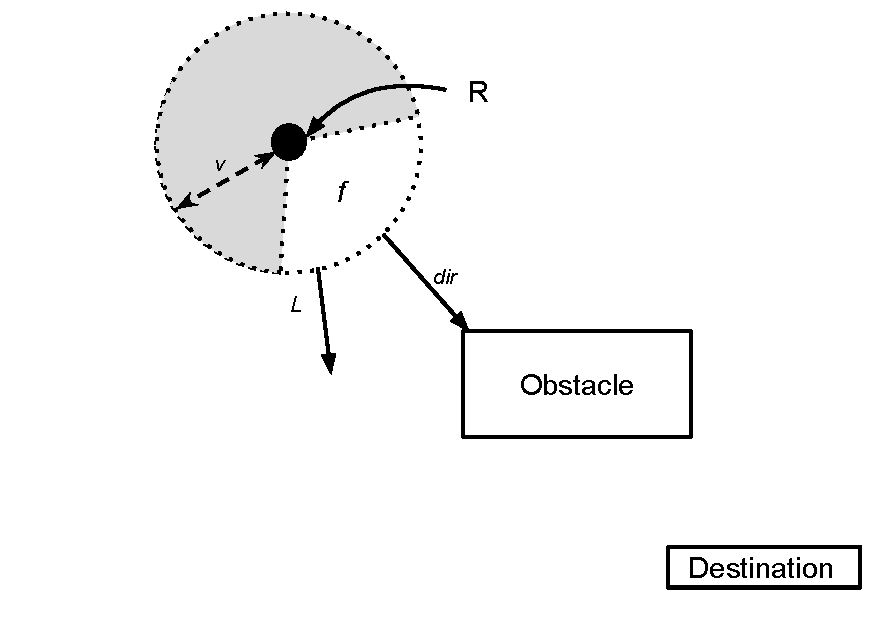
\includegraphics[width=0.75\textwidth]{chapters/chapter5/figures/ObstacleAvoidance.pdf}
	\caption{Navigation and Obstacle Avoidance, where $v$ is depth of view, $f$ is the field of view, $R$ is the robot, $dir$ is the direction of the destination and $L$ is a possible value of local attractor}
	\label{fig:obstacleavoidance}
\end{figure}


%%%%%%%%%%%%%%%%%%%%%%%%%%%%%%%%%%%%%%%%%%%%%%%%%
%%%%%%%%%%%%%%%%%%%%%%%%%%%%%%%%%%%%%%%%%%%%%%%%%
\section{Simulator}
\label{simulator}
A spatially discrete 2-dimensional grid world simulator has been developed and used in this thesis in order to accelerate computation \cite{sugawara2002swarming}. In real root experiments, algorithm performance is sensitive to the amount of time taken to load items and manoeuvre the robots \cite{ostergaard2001emergent}. The 2-dimensional grid world simulator allows for movement and loading time to be standardized across all algorithms for effective comparison.

The simulation robots function as follows:
\begin{itemize}
	\item Each robot fits into one grid block and each item takes up one grid block. 
	\item Only object can occupy a grid block at a time where an object is either a robot or an item. Since only one object can occupy a grid block at a time, collisions and congestion can occur.
	\item Each robot can move to an adjacent cell in any direction.
	\item Robots can load, transport and offload a single item at a time.
	\item If a robot does not pick up an item, the item is then an obstacle that a robot may have to navigate around in order to reach it's destination.
\end{itemize}

The prioritized and non-prioritized sinks were placed next to each other, on a single side of the environment. The sinks were marked by light beacons that all robots can detect and navigate towards. The reason the sinks were not placed in the centre of the environment, as is commonly found in swarm robotics research \cite{labella2006division}, is because the original prioritized foraging problem was inspired by the use of robots to forage gold and waste in mining tunnels. A mining tunnel has a single entrance where the gold and waste must be moved to, in order to be transported to the surface \cite{brune2010extracting}. Since there is only a single entrance at the beginning of a tunnel, the sinks need to occur at the beginning of the tunnel so that the items can be easily exported.

\section{Environments}
\label{experimentenvironments}

The experiments are to be run in different environments with different item distributions, sizes, item densities and different ratios of prioritized to non--prioritized items. 

The sizes of the environment grid, $S$, were varied, where $S\in \left\{ 50,100,200,300, 500\right\}$, such that $S$ was the width and length of the grid.  Experiments were run on different environment size to test how each algorithm can scale to larger environments.

Different values for the density of the items on the grid, $p$, were chosen where $p\in\left\{ 0.05, 0.2, 0.5, 0.7, 0.9\right\}$. Environments with a higher item density are more complex to forage since there exists a higher probability of an item on the unassigned type blocking the path to items of a robot's assigned type.

The ratio of prioritized to non-prioritized items $r$, was varied, where $r\in \left\{0, 0.2,0.25, 0.33, 0.5, 0.67, 0.75, 0.8, 1\right\}$. When no prioritized items on the grid existed, then $r=0$ and when only prioritized items on the grid existed, then $r=1$ .

In environments with a small $r$ value, the abundance of non-prioritized items increases the likelihood of non-prioritized items blocking the access to prioritized items. 

As $r$ is varied over varied, the swarm specialization ratio, $\tau$, is also varied, in order to determine of there exists a relationship between $r$, $\tau$ and the performance of the algorithms, in therms of $\sigma$. The parameter $r$ is also used to determine if the algorithms can adapt to the swarm specialization ratio, $\tau$, to optimally forage an environment of a given $r$. 

Different distributions of items over the environment were chosen to examine different characteristics of the algorithms. The item distributions are shown in Figure~\ref{fig:environments}, where each lighter shaded square is a prioritized item and a non-prioritized item is shown by a darker shaded square. Four different classes of environments were generated as follows:

\begin{enumerate}

\item The position of each item in a uniformly distributed environments are selected from a uniform distribution Environments (refer to Figure~\ref{fig:uniformenv}). The uniformly distributed environment has uniform concentrations of prioritized and non-prioritized items across the environment and thus is used as a control environment. 

\item For the Gaussian environments, the positions of the prioritized items are sampled from a Gaussian distribution, where the mean of the Gaussian function is the centre of the grid, and the distribution of the Gaussian function varies (refer to Figure~\ref{fig:gaussianenv}).

The positions of the non-prioritized items are selected after placing the prioritized items. The position for the non-prioritized items are selected from a uniform distribution. 

In Gaussian distributed environments, prioritized items  occur in high concentration in the center of the environment. More non-prioritized items occur on the outskirts of the environment, surrounding the prioritized items in the centre.

The Gaussian environments were used to examine whether each algorithm will enable the robot swarm to forage or navigate past the non-prioritized items to reach the high concentration of prioritized items in the environment's centre. 

\item Environments with a clustered items distribution have clusters of items of the same type (refer to Figure~\ref{fig:clusterenv}). The clusters were generated by Lumer-Faieta ant cemetery clustering \cite{lumer1994diversity}. After clusters have been generated, each cluster is labelled randomly as a either a cluster of prioritized items or a cluster of non-prioritized items. 

The goal of performing experiments in a clustered environment was to test an algorithms ability to exploit areas which are rich in prioritized items. Clustered environments were also be used to test how each algorithm can navigate around or forage non-prioritized items, as well as remember locations of areas which have a high density of prioritized items, in order to aid more efficient access to prioritized items. 

\item Environments with a vein distribution resemble the patterns observed in naturally occurring gold reefs \cite{frimmel2002recent} (refer to Figure~\ref{fig:veinenv}). In a gold reef, molten gold fills planar fractures between rock resulting in a vein of gold. Inspired by the gold reef, vein distributed environments have a long thin vein of prioritized items running from one side of the environment to another. The vein of prioritized items was surrounded by non-prioritized items. The non-prioritized items are similar to the rock surrounding the gold in gold reefs.

The vein environments aimed to test whether a swarm of robots, of each algorithm, could follow and forage the continuous length of the vein of prioritized items. A swarm that is able to detect the location of the vein and return to the vein's location after foraging an item should forage more than one that cannot detect and remember the location of the vein.

\end{enumerate} 

\begin{figure} [h]
        \centering
        \begin{subfigure}[b]{0.21\textwidth}
                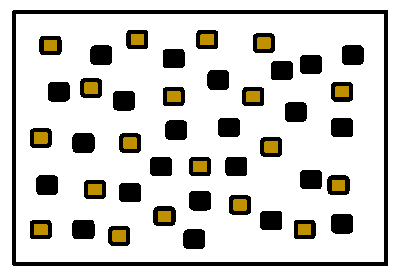
\includegraphics[width=\textwidth]{chapters/chapter4/figures/uniformenv.pdf}
                \caption{Uniform}
                \label{fig:uniformenv}
        \end{subfigure}%
        \begin{subfigure}[b]{0.205\textwidth}
                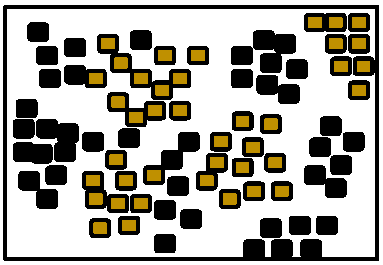
\includegraphics[width=\textwidth]{chapters/chapter4/figures/clusterenv.pdf}
                \caption{Clustered}
                \label{fig:clusterenv}
        \end{subfigure}
        \begin{subfigure}[b]{0.2\textwidth}
                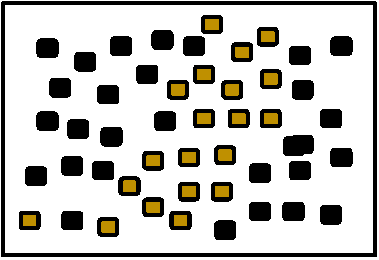
\includegraphics[width=\textwidth]{chapters/chapter4/figures/veinenv.pdf}
                \caption{Vein}
                \label{fig:veinenv}
        \end{subfigure}  
        \begin{subfigure}[b]{0.2\textwidth}
                        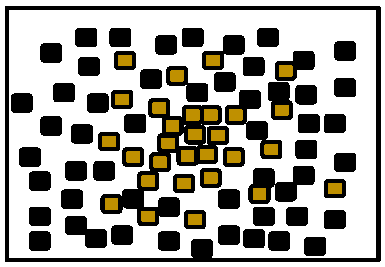
\includegraphics[width=\textwidth]{chapters/chapter4/figures/gaussianenv}
                        \caption{Gaussian}
                        \label{fig:gaussianenv}
       \end{subfigure}
        \caption{Environment Classes}\label{fig:environments}
\end{figure}


\begin{algorithm}

\caption{Uniform Distributed Environments}
\label{algorithm:uniform}
\begin{algorithmic}[1]
\Function{uniform}{numberitems, specializationratio, environmentsize}
\State \text{nonprioritizeditemsleft = floor((1-specializationratio)*numberitems)}
\State \text{prioritizeditemsleft = floor(specializationratio*numberitems)}
\While{\text{prioritizeditemsleft > 0}}
	\State \text{x $\gets$ uniform(0, environmentsize)}
	\State \text{y $\gets$ uniform(0, environmentsize)}
	\If{\text{position (x,y) is empty}}
		\State \text{Place prioritized item at (x,y)}
		\State \text{Decrement prioritizeditemsleft}
	\EndIf
\EndWhile

\While{\text{nonprioritizeditemsleft > 0}}
	\State \text{x $\gets$ uniform(0, environmentsize)}
	\State \text{y $\gets$ uniform(0, environmentsize)}
	\If{\text{position (x,y) is empty}}
		\State \text{Place prioritized item at (x,y)}
		\State \text{Decrement nonprioritizeditemsleft}
	\EndIf
\EndWhile
\EndFunction
\end{algorithmic}
\end{algorithm}


\begin{algorithm}

\caption{Gaussian Distributed Environments}
\label{algorithm:gaussian}
\begin{algorithmic}[1]
\Function{gaussian}{numberitems, specializationratio, environmentsize}
\State \text{calculate environment centre point (center_x, center_y)}
\State \text{prioritizeditemsleft = floor(specializationratio*numberitems)}
\State \text{nonprioritizeditemsleft = floor((1-specializationratio)*numberitems)}
\State \text{deviation = environmentsize*specializationratio/2}
\While{\text{prioritizeditemsleft > 0}}
	\State \text{x $\gets$ floor(gaussian(center_x, deviation)}
	\State \text{y $\gets$ floor(gaussian(center_y, deviation)}
	\If{\text{position (x,y) is empty and is valid}}
		\State \text{Place prioritized item at (x,y)}
		\State \text{Decrement prioritizeditemsleft}
	\EndIf
\EndWhile

\While{\text{nonprioritizeditemsleft > 0}}
	\State \text{x $\gets$ uniform(0, environmentsize)}
	\State \text{y $\gets$ uniform(0, environmentsize)}
	\If{\text{position (x,y) is empty}}
		\State \text{Place prioritized item at (x,y)}
		\State \text{Decrement nonprioritizeditemsleft}
	\EndIf
\EndWhile
\EndFunction
\end{algorithmic}
\end{algorithm}


\begin{algorithm}
\caption{Vein Distributed Environments}
\label{algorithm:vein}
\begin{algorithmic}[1]
\Function{vein}{numberitems, specializationratio, environmentsize}
\State \text{select 2 random sides from the grid}
\State \text{select a random points on each sides, $(x_0,y_0)$ and $(x_1,y_1)$}
\State \text{calculate gradient of vein, $m = (y_0 - y_1)/(x_0 - x_1)$}
\State \text{calculate $c$ of equation for line vein, $c = (y_0 - m*x_0)$
}

\State \text{prioritizeditemsleft = floor(specializationratio*numberitems)}
\State \text{nonprioritizeditemsleft = floor((1-specializationratio)*numberitems)}

\While{\text{prioritizeditemsleft > 0}}
	\State \text{x $\gets$ uniform($min(x_0,x_1), max(x_0, x_1)$)}
	\State \text{y $\gets m*x + c$}
	\If{\text{position (x,y) is valid and position (x,y) is empty}}
		\State \text{Place prioritized item at (x,y)}
		\State \text{Decrement prioritizeditemsleft}
	\EndIf
\EndWhile

\While{\text{nonprioritizeditemsleft > 0}}
	\State \text{x $\gets$ uniform(0, environmentsize)}
	\State \text{y $\gets$ uniform(0, environmentsize)}
	\If{\text{position (x,y) is empty}}
		\State \text{Place nonprioritized item at (x,y)}
		\State \text{Decrement nonprioritizeditemsleft}
	\EndIf
\EndWhile
\EndFunction
\end{algorithmic}
\end{algorithm}


\begin{algorithm}

%TODO
\caption{Clustered Distributed Environments}
\label{algorithm:uniform}
\begin{algorithmic}[1]
\Function{uniform}{numberitems, specializationratio, environmentsize}
\State \text{generate number of clusters, $totalclusters = uniform(3,15)$}
\State \text{Calculate number of prioritized clusters, $clusters_p = floor(specializationratio*totalclusters)$}
\State \text{Calculate number of non-prioritized clusters, $clusters_{np} = floor((1-specializationratio)*totalclusters)$}
\State \text{Calculate total number of prioritized items ,$total_p = floor(specializationratio*numberitems)$}
\State \text{Calculate total number of non-prioritized items ,$total_{np} = floor((1-specializationratio)*numberitems)$}
\State \text{Calculate average number of prioritized items per prioritized cluster, $ave_p = total_p/clusters_{p}$}
\State \text{Calculate average number of non-prioritized items per non-prioritized cluster, $ave_np = total_{np}/clusters_{np}$}
\State \text{$clusterstogenerate_p = clusters_p$}
\State \text{$clusterstogenerate_{np} = clusters_{np}$}

\While{\text{$clusterstogenerate_p > 0$}}
	\State \text{sample centroid for cluster $C$ (x,y) uniformly from grid}
	\State \text{sample random number of items, $num_p$ for cluster $C$ from uniform range ($ave_p/2$, $2ave_p$)}
	\State \text{Calculus radius, $r$, of cluster $C$ as $r = \sqrt{num_p/\pi}$}
	\If{\text{centroid (x,y) of cluster $C$ does not collide with boundaries of existing clusters}}
		\State \text{Save centroid and radius of cluster $C$ to list}
		\State \text{Decrement $clusterstogenerate_p$}
		\State \text{$itemstogenerate_p = num_p$}
				
		\While {$itemstogenerate_p > 0$}
			\State \text{Sample prioritized item position $(x_p,y_p)$ from Gaussian distribution with centre (x,y) and deviation $r$  }
			\If{\text{position $(x_{p},y_{p})$ is valid}}
				\State \text{Place prioritized item at $(x_p,y_p)$}
				\State \text{Decrement $itemstogenerate_{np}$}	
			\EndIf
		\EndWhile
	\EndIf
	\EndIf
\EndWhile

\While{\text{$clusterstogenerate_{np} > 0$}}
	\State \text{sample centroid for cluster $C$ (x,y) uniformly from grid}
	\State \text{sample random number of items, $num_{np}$ for cluster $C$ from uniform range ($ave_{np}/2$, $2ave_{np}$)}
	\State \text{Calculus radius, $r$, of cluster $C$ as $r = \sqrt{num_{np}/\pi}$}
	\If{\text{centroid (x,y) of cluster $C$ does not collide with boundaries of existing clusters}}
	
		\State \text{Save centroid and radius of cluster $C$ to list}
		\State \text{Decrement $clusterstogenerate_{np}$}
		\State \text{$itemstogenerate_{np} = num_{np}$}
				
		\While {$itemstogenerate_{np} > 0$}
			\State \text{Sample prioritized item position $(x_{np},y_{np})$ from Gaussian distribution with centre (x,y) and deviation $r$  }
			\If{\text{position $(x_{np},y_{np})$ is valid}}
				\State \text{Place non-prioritized item at $(x_{np},y_{np})$}
				\State \text{Decrement $itemstogenerate_{np}$}	
			\EndIf
		\EndWhile
	\EndIf
	\EndIf
\EndWhile

\EndFunction
\end{algorithmic}
\end{algorithm}

\section{Swarm Parameters}
\label{parameters}

For all algorithms, the robot swarm was initialized with 
some swarm specialization ratio, $\tau$ where $\tau\in\left\{0, 0.2, 0.25, 0.333, 0.5, 0.667, 0.75, 0.8,1\right\}$. The swarm specialization ratio is ratio of robots foraging prioritized items to non-prioritized items. When no robots are set to initially forage prioritized items then $tau=0$ and when all robots are set to initially forage prioritized items then $tau=1$.

As discussed in Section~\ref{experimentenvironments}, $\tau$ is varied, with a specific $r$, to determine if the ratio of $\tau$ to $r$ has an effect on algorithm performance. Also, the ability of an algorithm to adapt the value of $\tau$ appropriately for a given $r$, indicates the flexibility of an algorithm. %Why? How?

The density of robots, $c$, is defined as the density of cells, of the grid size $S$ (the length of the side of an environment) that are occupied by robots, where $c\in\left\{0.1, 0.3, 0.5, 0.7, 1\right\}$. The density of robots is varied in order to test the scalability of the algorithm. The density of robots is also varied to test each algorithms' ability to adjust the amount of actively  foraging robots to the density of the items in the environment.

The honey bee algorithm specific parameters were selected based on \cite{seeley2009wisdom}, where
-$t_{max}=200$ time steps, $f_{max}=100$ time steps, $\phi=0.8$ and $\rho=0.1$. Testing the effect of each of the honey bee algorithm specific parameters was not in the scope of this thesis.

The initial position of each robot was randomly selected, adjacent to the sink. All robots began in the exploration state, which a state that is shared by all algorithms. For each set of algorithmic, environmental and swarm configurations, each simulation was run for 10000 time steps. An experiment consists of 30 repeated simulations for a specific set of parameters.

\section{Performance Measures}
\label{thri:third:performancemeasures}

%What do I need to add to 
%TODO: The idea is to add more robots foraging the prioritized items.
The following performance measures were used: 

	\begin{itemize}
		\item	The percentage of prioritized items foraged over time,  $\sigma$ 
		\item	The percentage of non-prioritized items foraged over time, $\mu$
		\item   The average time spent by agents waiting at the sink, $\epsilon$
	\end{itemize}
	
Future studies could include the average time taken by a robot to forage an item, the average distance moved by a robot and a measure to explain the randomness of a robots movement, but are not addressed in this thesis. 



%%%%%%%%%%%%%%%%%%%%%%%%%%%%%%%%%%%%%%%%%%%%%%%%%

%%%%%%%%%%%%%%%%%%%%%%%%%%%%%%%%%%%%%%%%%%%%%%%%%
%%%%%%%%%%%%%%%%%%%%%%%%%%%%%%%%%%%%%%%%%%%%%%%%%
%%%%%%%%%%%%%%%%%%%%%%%%%%%%%%%%%%%%%%%%%%%%%%%%%
%%%%%%%%%%%%%%%%%%%%%%%%%%%%%%%%%%%%%%%%%%%%%%%%%
\section{Summary}
\label{third:summary}
The robots used in this study are based on the e-puck robots, but with gripper capabilities. The robots used a navigation and obstacle avoidance technique based on the flocking behaviour of birds where a global attractor force attracts the robot in a specific direction, while the local attractor force guide the robot around localized obstacles. A simple 2-dimensional grid-based simulator is used. Only a single robot or item could occupy a single grid cell at once.

The environment types, that were generated for experimentation in order to test different properties of the algorithms were discussed. The environment types defined have the four following distributions: uniform distribution, Gaussian distribution, clustered distribution and vein distribution. The following environmental parameters were varied: item density, environment size and item type ratio. The following swarm parameters chosen for each of the algorithms were presented: initial swarm configuration, swarm density, and honey bee specific parameters. Performance measures were selected to compare different aspects of the algorithms: the different percentages of each type of item foraged as well as the time spent waiting by the sink. 

%%%
%%%%%%%%%%%%%%%%%%%%%%%%%%%%%%%%%%%%%%%%%%%%%%%%%
%%%%%%%%%%%%%%%%%%%%%%%%%%%%%%%%%%%%%%%%%%%%%%%%%